\documentclass[conference]{IEEEtran}
\IEEEoverridecommandlockouts

\usepackage{cite}
\usepackage{amsmath,amssymb,amsfonts}
\usepackage{algorithmic}
\usepackage{graphicx}
\usepackage{textcomp}
\usepackage{xcolor}
\usepackage{float}
\usepackage{listings}

\lstset{
    basicstyle=\small\ttfamily,     % Tamaño de fuente pequeño y fuente monoespaciada
    breaklines=true,                % Permite dividir líneas largas
    columns=fullflexible,           % Permite que las líneas se ajusten al ancho del texto
    frame=single,                   % Añade un marco alrededor del código
    language=Python,                % Lenguaje de programación
    numbers=left,                   % Números de línea a la izquierda
    numberstyle=\tiny,              % Tamaño de fuente de los números de línea
    xleftmargin=1em,                % Margen izquierdo
}

\title{Análisis de Componentes Principales}

\author{
\IEEEauthorblockN{Portilla Posadas F. D.\textsuperscript{1}}
\IEEEauthorblockA{
\textit{Ingeniería en Inteligencia Artificial} \\
\textit{Unidad Profesional Interdisciplinaria de Ingeniería, Campus Tlaxcala, Instituto Politécnico Nacional}\\
Tlaxacala, México\\
fportillap2100@alumno.ipn.mx
}
}

\begin{document}
\maketitle

\begin{abstract}
    En esta práctica, exploraremos el Análisis de Componentes Principales (PCA) como una técnica fundamental para reducir la dimensionalidad de conjuntos de datos multivariados. Nuestro enfoque se centrará en su aplicación práctica en el contexto del conocido conjunto de datos Iris. A través de esta práctica, aprenderemos a cargar y normalizar los datos, calcular los componentes principales y determinar el número óptimo de componentes. Al final del proceso, seremos capaces de visualizar los datos en un espacio bidimensional, lo que facilitará la identificación de patrones y relaciones entre las diferentes especies de iris.
\end{abstract}

\section{Introducción}

El PCA es una herramienta poderosa para simplificar conjuntos de datos complejos al transformar variables originales en componentes principales ortogonales que capturan la variabilidad de los datos. Esto es especialmente útil en la visualización de datos, la eliminación de ruido y la simplificación de modelos. A través de esta práctica, desarrollaremos un entendimiento práctico del PCA y cómo aplicarlo en el contexto de los datos del conjunto de Iris.

\section{Marco Teórico}

\subsection{Análisis de componentes principales (PCA)}
El Análisis de Componentes Principales (PCA) es una técnica estadística que se utiliza para reducir la dimensionalidad de los datos multivariados. Su objetivo principal es transformar un conjunto de variables originales en un nuevo conjunto de variables llamadas componentes principales. Estos componentes son combinaciones lineales de las variables originales y están diseñados para ser ortogonales entre sí.

El PCA se basa en la matriz de covarianza de las variables originales, que muestra las relaciones de covarianza entre ellas. Los componentes principales se obtienen de manera que el primer componente capture la mayor varianza en los datos, el segundo componente capture la segunda mayor varianza y así sucesivamente. Esto permite resumir la información contenida en muchas variables en un conjunto más pequeño de variables no correlacionadas.

La reducción de dimensionalidad es una de las aplicaciones más importantes del PCA. Al proyectar los datos en el espacio de los componentes principales y seleccionar un número menor de componentes, es posible simplificar la representación de los datos mientras se conserva la mayor parte de la variabilidad. Esto es útil para la visualización de datos, la eliminación de ruido y la simplificación de modelos en diversos campos.

\subsection{Conjunto de datos Iris}

El conjunto de datos Iris es un conjunto de datos ampliamente utilizado en estadísticas y aprendizaje automático para ilustrar diversas técnicas y algoritmos. Fue introducido por el biólogo y estadístico británico Ronald A. Fisher en 1936 y consta de 150 muestras de iris de tres especies diferentes: Iris setosa, Iris versicolor e Iris virginica. Cada especie se describe mediante cuatro características: la longitud del sépalo, el ancho del sépalo, la longitud del pétalo y el ancho del pétalo.

Este conjunto de datos es un ejemplo ideal para aplicar técnicas de clasificación y reducción de dimensionalidad, como el Análisis de Componentes Principales (PCA). El PCA se utiliza para reducir la dimensionalidad de las cuatro características originales a un número menor de componentes principales, lo que facilita la visualización de las diferencias entre las especies de iris y la clasificación de nuevas muestras.


\section{Desarrollo}

El conjunto de datos se carga usando la librería Pandas de Python, esto se hace con la finalidad de graficar fácilmente los datos y poder manipularlos de una manera más sencilla.

El conjunto consta de 150 registros de flores, cada registro describe una flor con 4 características: longitud del sépalo, ancho del sépalo, longitud del pétalo y ancho del pétalo. Cada registro también contiene la especie de la flor, que puede ser Iris setosa, Iris versicolor o Iris virginica. Además se hace una normalización de la distribución de los datos, esto se hace con la finalidad de que los datos tengan una distribución normal y así poder aplicar el PCA.

\begin{lstlisting}[language=Python, caption=Carga de datos y normalización]

#Se lee el archivo iris.data
iris = pd.read_csv('iris.data', header=None)

#Se asignan los nombres de las columnas
iris.columns = ['sepal_length', 'sepal_width', 'petal_length', 'petal_width', 'class']

#Se separan los datos de las etiquetas
X = iris.iloc[:,0:4].values
y = iris.iloc[:,4].values

#Se normalizan los datos
from sklearn.preprocessing import StandardScaler
X_std = StandardScaler().fit_transform(X)
\end{lstlisting}

El siguiente paso es aplicar PCA para reducir la dimensionalidad del conjunto de datos. Para este paso se usó la librería Scikit-learn de Python, la cual contiene una implementación de PCA. 

\begin{lstlisting}[language=Python, caption=Aplicación de PCA]
    #Se aplica PCA a los datos normalizados
from sklearn.decomposition import PCA as sklearnPCA
sklearn_pca = sklearnPCA(n_components=4)
Y_sklearn = sklearn_pca.fit_transform(X_std)
\end{lstlisting}

El método para determinar la cantidad de componenetes principales es la varianza acumulada, la cual se calcula con la siguiente fórmula:

\begin{equation}
    \frac{\sum_{i=1}^{n} \lambda_{i}}{\sum_{i=1}^{p} \lambda_{i}} \geq 0.95
\end{equation}

Donde $\lambda_{i}$ es el valor propio de la matriz de covarianza y $p$ es el número de componentes principales.

En el siguiente fragmento de código se calcula la varianza acumulada y se grafica para determinar el número de componentes principales.

\begin{lstlisting}[language=Python, caption=Varianza acumulada]
    #La varianza total es la suma de las varianzas de cada componente original
    total_var = np.sum(eig_vals)
    print('Varianza total \n%s' %total_var)
    
    #Se calcula la varianza acumulada
    var_acum = np.cumsum(eig_vals)/total_var

\end{lstlisting}

Finalmente para visualizar los resultados, nuevamente haciendo uso de Pandas se grafican los datos originales, además de los datos transformados por PCA.
\begin{lstlisting}[language=Python, caption=Graficación de datos]
    #Se visualizan los datos en 2 dimensiones
    pd.plotting.scatter_matrix(iris, figsize=(10,10))
    plt.show()
    
    # Define a mapping of labels to colors
    label_to_color = {
        'Iris-setosa': 'red',
        'Iris-versicolor': 'blue',
        'Iris-virginica': 'green'
    }
    
    # Assuming 'y' contains the labels for your data points
    colors = [label_to_color[label] for label in y]
    
    # Now you can create the scatter plot
    plt.scatter(Y_sklearn[:, 0], Y_sklearn[:, 1], c=colors)
    plt.xlabel('Componente principal 1')
    plt.ylabel('Componente principal 2')
    plt.title('Visualizacion de los datos en 2 dimensiones')
    plt.show()

\end{lstlisting}

\section{Resultados}

\begin{figure}[H]
    \centering
    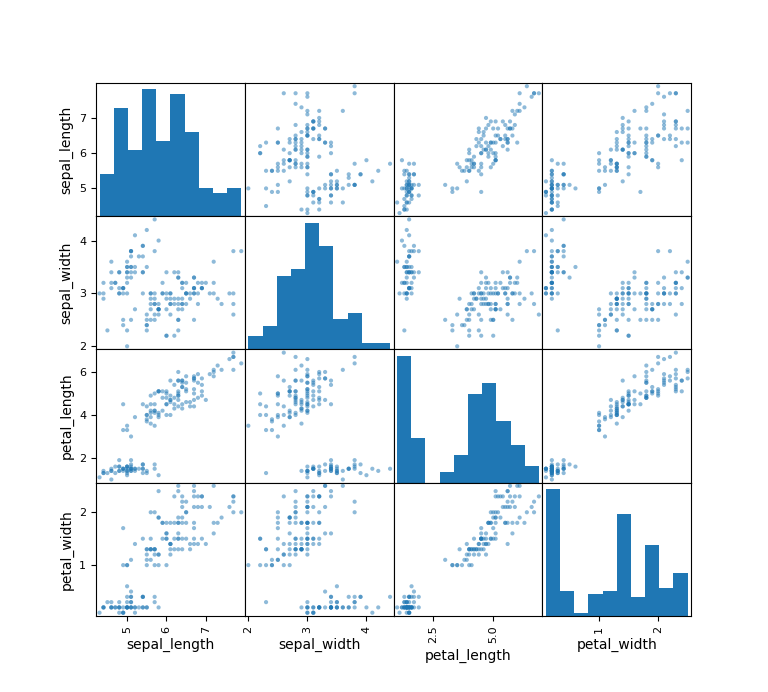
\includegraphics[width=0.5\textwidth]{images/originales.png}
    \caption{Datos originales}
    \label{fig:my_label}
\end{figure}




\begin{table}[H]
\centering
\caption{Valores propios y varianza acumulada}
\label{my-label}
\begin{tabular}{|l|l|l|}
\hline
\textbf{Componente} & \textbf{Valor propio} & \textbf{Varianza acumulada} \\ \hline
1                   & 2.93035378            & 0.72770452                  \\ \hline
2                   & 0.92740362            & 0.95800975                  \\ \hline
3                   & 0.14834223            & 0.99479538                  \\ \hline
4                   & 0.02074601            & 1                           \\ \hline
\end{tabular}
\end{table}

\begin{figure}[H]
    \centering
    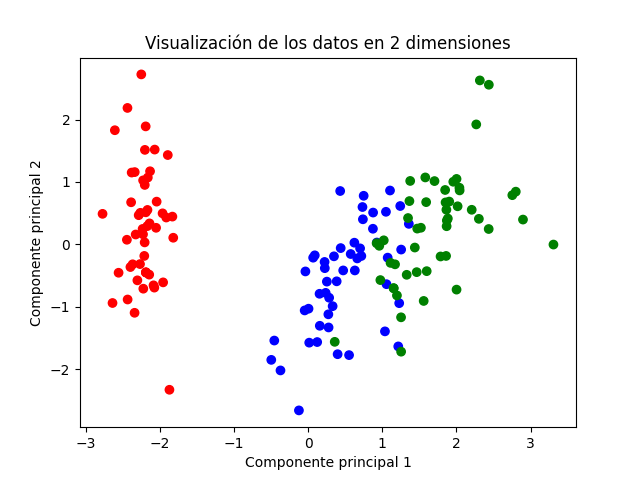
\includegraphics[width=0.5\textwidth]{images/pca.png}
    \caption{Datos transformados por PCA}
    \label{fig:my_label}
\end{figure}




\subsection{Análisis de resultados}
Como se puede visualizar en las figuras 1 y 2, los datos originales se encuentran en un espacio de 4 dimensiones, por lo que es difícil visualizarlos. En la figura 3 se puede observar que los datos se encuentran en un espacio de 2 dimensiones, esto es gracias a la reducción de dimensionalidad que se hizo con PCA.

La tabla 1 muestra los valores propios y la varianza acumulada de los datos originales. Como se puede observar, es posible reducir la dimensionalidad de los datos a 2 dimensiones y conservar el 95\% de la varianza.

\section{Conclusiones}

Es posible hacer una reducción en la dimensionalidad de los datos mediante el uso de PCA, esto es útil para poder visualizar los datos y poder aplicar algoritmos de clasificación. Al hacer un análisis estadístico de los datos, se puede determinar la cantidad de componentes principales que se deben usar para conservar la mayor cantidad de varianza posible, es decir, que los datos aún puedan ser representativos.

\begin{thebibliography}{00}
\bibitem{b2}  Principal Component Analysis in Python, Datacamp, https://www.datacamp.com/community/tutorials/principal-component-analysis-in-python
\end{thebibliography}


\end{document}
